\documentclass  [12pt]{article}
\usepackage{graphicx}


\begin{document}


Dana Idák\cite{1}
\begin{document}

\begin{titlepage}
    \maketitle
\end{titlepage}




\begin{figure}
\begin{center}
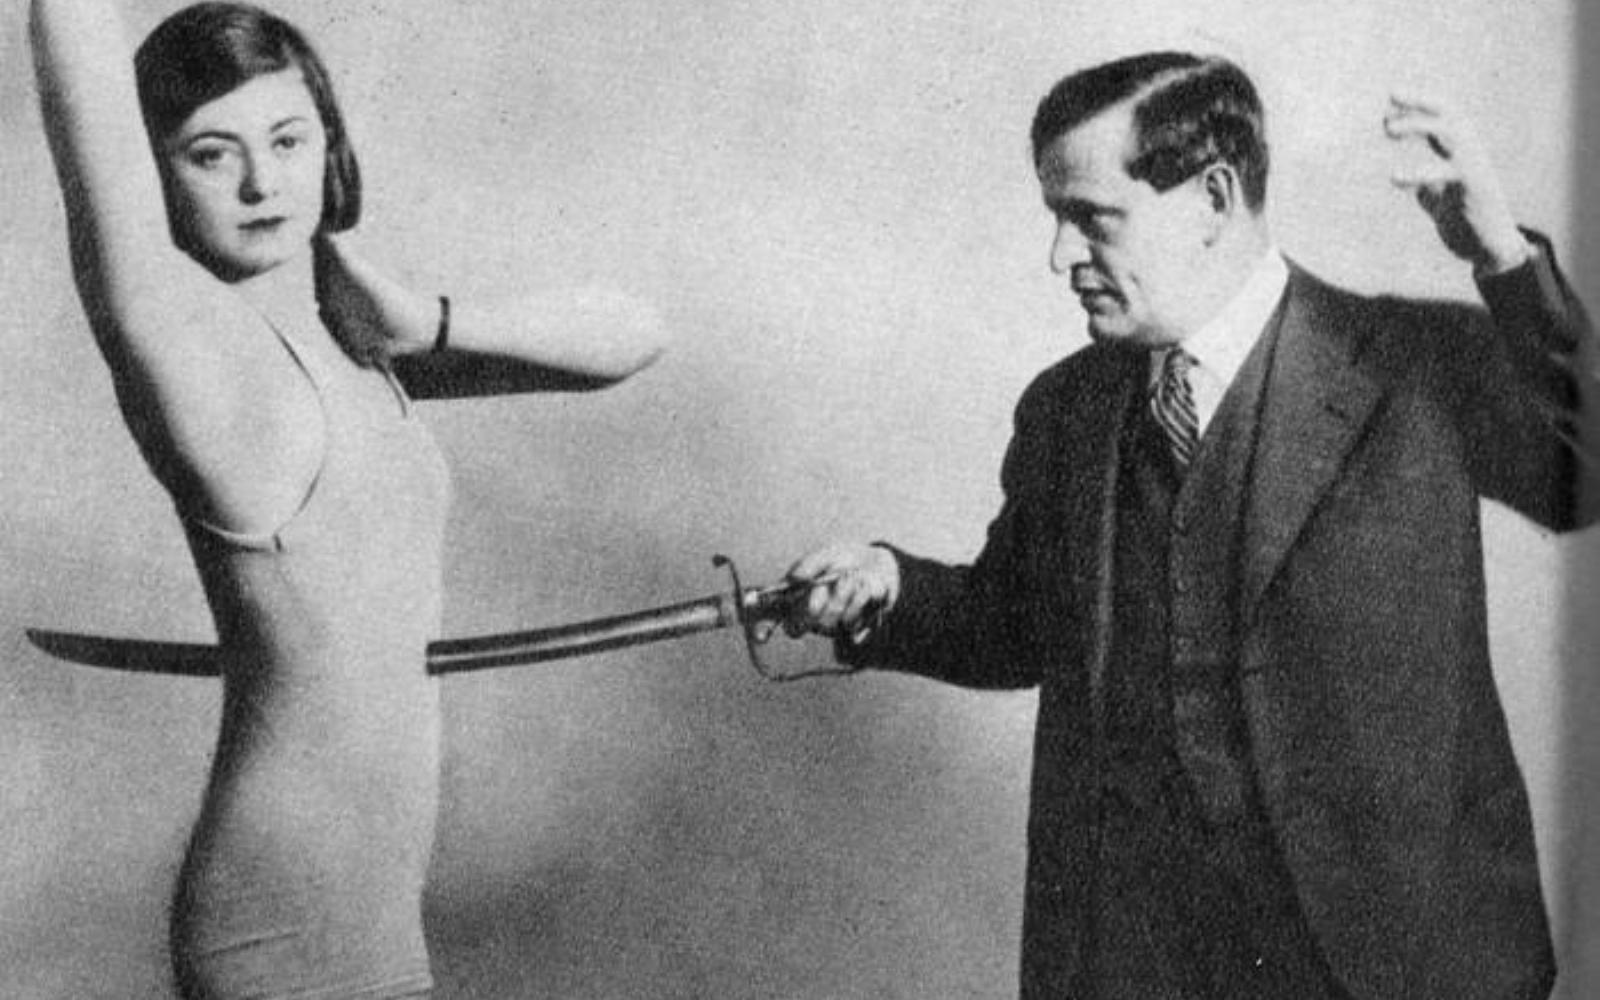
\includegraphics[angle=5, width=5cm]{igy_irtok_ti.jpeg}
\end{center}
\end{figure}


\footnote{Matematikai költemény.}

Lent a lenső lélekuton \{Hádesz öblén, [hol a lélek élet – állott (élet – állott, mint az állat) s aspodélosz illatokkal] öblögetve, ablakokba\} ablakokba öblögetve, öblögekbe ablakogva és makogva mekegve.\\


És mekegve és makogva lent a mélybe, lent $ \sqrt[2]{lent}  $ az éjbe, hol a kéjbe $ {ejbe,melybe \choose   kejbe,ejbe} $.

Ötven asszony, logarithmus ötven asszony és emelve és kivonva, négyzetekre köbgyökökre, ötven asszony, hetven asszony, százhuszonhét bűnös asszony, ötven órjás amphorába, asfodélosz ötven asszony = bünös asszony, mennyi jött ki, mennyi jött ki.\\
Százkilencven bűnös asszony, óriási amphorába, amphorába \begin{math} \sqrt[2]{amphoraba} \end{math} , rába, rába, rába, majd mekegve, $(\log) $ majd makogva, mindörökre, mindhiába, (mert hiába [mind hiába] töltögetve, öblögetve) öblögetve ablakokba, ablagokva, és makogva,\begin{displaymath} (oblogekbe)^{2} \end{displaymath} és mekegve és makogva, fogjanak $ \sqrt[2]{fogjanak} $ meg, fogjanak meg…\\

\begin{center}
(Megfogják.)
\end{center}

\pagebreak



Struggle for life  \cite{2}

\begin{titlepage}
    \maketitle
\end{titlepage}


Pajtás, úgy fest, alulmaradtál
A Tétel és Törvény szerint –
Dögödre már hiéna szaglász
S a varjú éhesen kering.
Nem is a falka volt erősebb
Apró vadak tángáltak el –
S hogy írhádon ki osztozik most
Véreb? Veréb? Nem érdekel.
Öklöd, mikor lecsapni kellett
Mindig megállt a féluton –
Jóság volt? Gyöngeség? Nem értem.
Félsz? Gőg? Szemérem? Nem tudom.
Talán csak undor. Jól van így is.
Megnyugszom. Ámen. Úgy legyen.
Inkább egyenek meg a férgek
Minthogy a férget megegyem.\\

\bibitem{1} KARINTHY F.: Így írtok ti 1912

\bibitem{2} KARINTHY F.: Üzenet a palackban 1930



\end{document}
